%===========================================================
% This is the thesis template for the Statistics major at
% Amherst College. Brittney E. Bailey (bebailey@amherst.edu)
% adapted this template from the Reed College LaTeX thesis
% template in January 2019 with major updates in April 2020.
% Please send any comments/suggestions: bebailey@amherst.edu

% Most of the work for the original document class was done
% by Sam Noble (SN), as well as this template. Later comments
% etc. by Ben Salzberg (BTS). Additional restructuring and
% APA support by Jess Youngberg (JY). Email: cus@reed.edu
%===========================================================

\documentclass[12pt, twoside]{amherstthesis}
\usepackage{graphicx,latexsym}
\usepackage{amsmath}
\usepackage{amssymb,amsthm}
\usepackage{longtable,booktabs} %setspace loaded in .cls
\usepackage[hyphens]{url}
\usepackage{hyperref}
\usepackage{lmodern}
\usepackage{float}
\floatplacement{figure}{H}
\usepackage{rotating}
\usepackage{fancyvrb}
% User-added packages:
% End user-added packages

%===========================================================
% BIBLIOGRAPHY FORMATTING

% Next line commented out by CII
%%% \usepackage{natbib}
% Comment out the natbib line above and uncomment the
% following two lines to use the new biblatex-chicago style,
% for Chicago A. Also make some changes at the end where the
% bibliography is included.
%\usepackage{biblatex-chicago}
%\bibliography{thesis}


%===========================================================
% HYPERLINK FORMATTING

% Added by CII (Thanks, Hadley!)
% Use ref for internal links
\renewcommand{\hyperref}[2][???]{\autoref{#1}}
\def\chapterautorefname{Chapter}
\def\sectionautorefname{Section}
\def\subsectionautorefname{Subsection}
% End of CII addition
\usepackage{xcolor}
\hypersetup{
    colorlinks,
    linkcolor={red!50!black},
    citecolor={blue!50!black},
    urlcolor={blue!80!black}
}

%===========================================================
% CAPTION FORMATTING

% Added by CII
\usepackage{caption}
\captionsetup{width=5in}
% End of CII addition

%===========================================================
% TITLE FORMATTING

\renewcommand{\contentsname}{Table of Contents}

\usepackage{titlesec}
%%%%%%%%
% How to use titlesec:
% \titleformat{⟨command⟩}[⟨shape⟩]{⟨format⟩}{⟨label⟩}{⟨sep⟩}
%  {⟨before-code⟩}[⟨after-code⟩]
%%%%%%%%

\titleformat{\chapter}[hang]
{\normalfont%
    \Large% %change this size to your needs for the first line
    \bfseries}{\chaptertitlename\ \thechapter}{1em}{%
      %change this size to your needs for the second line
    }[]

\titleformat{\section}[hang]
{\normalfont%
    \large % %change this size to your needs for the first line
    \bfseries}{\thesection}{1em}{%
     %change this size to your needs for the second line
    }[]

\titleformat{\subsection}[hang]
{\normalfont%
    \normalsize % %change this size to your needs for the first line
    \bfseries}{\thesubsection}{1em}{%
     %change this size to your needs for the second line
    }[]

% \titleformat{\section}[display]
% {\normalfont%
%     \large% %change this size to your needs for the first line
%     \bfseries}{\chaptertitlename\ \thechapter}{20pt}{%
%     \normalsize %change this size to your needs for the second line
%     }


%===========================================================
% DOCUMENT FONT

% \usepackage{times}
% other fonts available eg: times, bookman, charter, palatino


%===========================================================
% PASSING FORMATS FROM RMD --> LATEX

%%%%%%%%
% NOTE: Dollar signs pass parameters between YAML inputs
% in index.Rmd and LaTeX
%%%%%%%%

\Abstract{
The abstract should be a short summary of your thesis work. A paragraph is usually sufficient here.
}

\Acknowledgments{
Use this space to thank those who have helped you in the thesis process (professors, staff, friends, family, etc.). If you had special funding to conduct your thesis work, that should be acknowledged here as well.
}

\Dedication{

}

\Preface{

}

% Formatting R code display
% Syntax highlighting #22
  \usepackage{color}
  \usepackage{fancyvrb}
  \newcommand{\VerbBar}{|}
  \newcommand{\VERB}{\Verb[commandchars=\\\{\}]}
  \DefineVerbatimEnvironment{Highlighting}{Verbatim}{commandchars=\\\{\}}
  % Add ',fontsize=\small' for more characters per line
  \usepackage{framed}
  \definecolor{shadecolor}{RGB}{248,248,248}
  \newenvironment{Shaded}{\begin{snugshade}}{\end{snugshade}}
  \newcommand{\AlertTok}[1]{\textcolor[rgb]{0.94,0.16,0.16}{#1}}
  \newcommand{\AnnotationTok}[1]{\textcolor[rgb]{0.56,0.35,0.01}{\textbf{\textit{#1}}}}
  \newcommand{\AttributeTok}[1]{\textcolor[rgb]{0.77,0.63,0.00}{#1}}
  \newcommand{\BaseNTok}[1]{\textcolor[rgb]{0.00,0.00,0.81}{#1}}
  \newcommand{\BuiltInTok}[1]{#1}
  \newcommand{\CharTok}[1]{\textcolor[rgb]{0.31,0.60,0.02}{#1}}
  \newcommand{\CommentTok}[1]{\textcolor[rgb]{0.56,0.35,0.01}{\textit{#1}}}
  \newcommand{\CommentVarTok}[1]{\textcolor[rgb]{0.56,0.35,0.01}{\textbf{\textit{#1}}}}
  \newcommand{\ConstantTok}[1]{\textcolor[rgb]{0.00,0.00,0.00}{#1}}
  \newcommand{\ControlFlowTok}[1]{\textcolor[rgb]{0.13,0.29,0.53}{\textbf{#1}}}
  \newcommand{\DataTypeTok}[1]{\textcolor[rgb]{0.13,0.29,0.53}{#1}}
  \newcommand{\DecValTok}[1]{\textcolor[rgb]{0.00,0.00,0.81}{#1}}
  \newcommand{\DocumentationTok}[1]{\textcolor[rgb]{0.56,0.35,0.01}{\textbf{\textit{#1}}}}
  \newcommand{\ErrorTok}[1]{\textcolor[rgb]{0.64,0.00,0.00}{\textbf{#1}}}
  \newcommand{\ExtensionTok}[1]{#1}
  \newcommand{\FloatTok}[1]{\textcolor[rgb]{0.00,0.00,0.81}{#1}}
  \newcommand{\FunctionTok}[1]{\textcolor[rgb]{0.00,0.00,0.00}{#1}}
  \newcommand{\ImportTok}[1]{#1}
  \newcommand{\InformationTok}[1]{\textcolor[rgb]{0.56,0.35,0.01}{\textbf{\textit{#1}}}}
  \newcommand{\KeywordTok}[1]{\textcolor[rgb]{0.13,0.29,0.53}{\textbf{#1}}}
  \newcommand{\NormalTok}[1]{#1}
  \newcommand{\OperatorTok}[1]{\textcolor[rgb]{0.81,0.36,0.00}{\textbf{#1}}}
  \newcommand{\OtherTok}[1]{\textcolor[rgb]{0.56,0.35,0.01}{#1}}
  \newcommand{\PreprocessorTok}[1]{\textcolor[rgb]{0.56,0.35,0.01}{\textit{#1}}}
  \newcommand{\RegionMarkerTok}[1]{#1}
  \newcommand{\SpecialCharTok}[1]{\textcolor[rgb]{0.00,0.00,0.00}{#1}}
  \newcommand{\SpecialStringTok}[1]{\textcolor[rgb]{0.31,0.60,0.02}{#1}}
  \newcommand{\StringTok}[1]{\textcolor[rgb]{0.31,0.60,0.02}{#1}}
  \newcommand{\VariableTok}[1]{\textcolor[rgb]{0.00,0.00,0.00}{#1}}
  \newcommand{\VerbatimStringTok}[1]{\textcolor[rgb]{0.31,0.60,0.02}{#1}}
  \newcommand{\WarningTok}[1]{\textcolor[rgb]{0.56,0.35,0.01}{\textbf{\textit{#1}}}}

% Formatting R code: set baselinestretch = 1.5 for double-spacing
\DefineVerbatimEnvironment{Highlighting}{Verbatim}{
  baselinestretch = 1,
  commandchars=\\\{\}}

% Formatting R output display: set baselinestretch = 1.5 for double-spacing
\DefineVerbatimEnvironment{verbatim}{Verbatim}{
  baselinestretch = 1,
  % indent from left margin
  xleftmargin = 1mm,
  % vertical grey bar on left side of R output
  frame = leftline,
  framesep = 0pt,
  framerule = 1.5mm, rulecolor = \color{black!15}
  }

\title{My amazing title}
\author{Your R. Name}
\date{April DD, 20YY}
\division{}
\advisor{Advisor F. Name}
% for second advisor
\institution{Amherst College}
\degree{Bachelor of Arts}
\department{Mathematics and Statistics}

% Fix from pandoc about cslreferences?
% https://github.com/mpark/wg21/issues/54

% Added by CII
%%% Copied from knitr
%% maxwidth is the original width if it's less than linewidth
%% otherwise use linewidth (to make sure the graphics do not exceed the margin)
\makeatletter
\def\maxwidth{ %
  \ifdim\Gin@nat@width>\linewidth
    \linewidth
  \else
    \Gin@nat@width
  \fi
}
\makeatother

% ===========================================
% DOCUMENT SPACING

\setlength{\parskip}{0pt}
% Added by CII

\providecommand{\tightlist}{%
  \setlength{\itemsep}{0pt}\setlength{\parskip}{0pt}}


% ===========================================
% ===========================================
% ===========================================
\usepackage{amsthm}
\newtheorem{theorem}{Theorem}[chapter]
\newtheorem{lemma}{Lemma}[chapter]
\newtheorem{corollary}{Corollary}[chapter]
\newtheorem{proposition}{Proposition}[chapter]
\newtheorem{conjecture}{Conjecture}[chapter]
\theoremstyle{definition}
\newtheorem{definition}{Definition}[chapter]
\theoremstyle{definition}
\newtheorem{example}{Example}[chapter]
\theoremstyle{definition}
\newtheorem{exercise}{Exercise}[chapter]
\theoremstyle{remark}
\newtheorem*{remark}{Remark}
\newtheorem*{solution}{Solution}
\begin{document}

\doublespace
% Everything below added by CII
  \maketitle

\frontmatter % this stuff will be roman-numbered
\pagenumbering{roman}
\pagestyle{fancyplain}
%\pagestyle{fancy} % this removes page numbers from the frontmatter

  \begin{abstract}
    The abstract should be a short summary of your thesis work. A paragraph is usually sufficient here.
  \end{abstract}
  \begin{acknowledgments}
    Use this space to thank those who have helped you in the thesis process (professors, staff, friends, family, etc.). If you had special funding to conduct your thesis work, that should be acknowledged here as well.
  \end{acknowledgments}

  \hypersetup{linkcolor=black}
  \setcounter{tocdepth}{2}
  \tableofcontents

  \addcontentsline{toc}{chapter}{List of Tables}\listoftables

  \addcontentsline{toc}{chapter}{List of Figures}\listoffigures


\mainmatter % here the regular arabic numbering starts
\pagenumbering{arabic}
\pagestyle{fancyplain} % turns page numbering back on

\hypertarget{intro}{%
\chapter{Introduction}\label{intro}}

In standard undergraduate curricula, there is a strong focus on cross sectional data, and thus no emphasis on how time-sequence data is analyzed. However, a significant portion of data that we encounter in the real world is dependent on time. If we want to track trends and changes over time, such as an effect of a certain drug on the body or growth of a company, longitudinal data and analysis will help us examine those points of interest. For example, the Chinese Longitudinal Healthy Longevity Survey from Duke University assessed physical and mental well-being of Chinese elders for over almost 2 decades and re-interviewed survivors every few year. This follow up in data collection allowed researchers to investigate the aging process over time and identify risk factors and causes leading up to death.

Not only can we observe change over time in individuals, but we can look at higher-level grouping, such as change in schools, counties, and organizations. It should be emphasized that only longitudinal data can capture changes within a subject or group; cross-sectional data contain responses that are captured at only one occasion that are then compared to other subjects. Ultimately, it cannot provide information about changes over time.

One key aspect of longitudinal data is that there needs to be repeated measurements of the same individuals across multiple periods of time. If there aren't repeated observations, then it is not possible to make any comparisons between two or more time points. Having repeated measurements of the same individual allows for removal of potential confounding effects, such as gender or socioeconomic status, from the analysis. Since we assume that these confounding variables are fixed effects that do not vary from measurement to measurement, all changes from an individual cannot be attributed to these effects.

The measure that captures the observed changes within an individual is referred to as a response trajectory. There are different ways of comparing response trajectories. For example, it is possible to compare the post-treatment vs baseline changes across multiple treatment groups, or it is also possible to compare the rate of change. The method chosen depends on the specific question of the study.

Apart from comparing just the response trajectories, it is also of interest to compare individual differences in the relationship between covariates and the response trajectory. This can be captured using various different statistical models. The choice of model depends on several characteristics of the data.

\hypertarget{characteristics-of-longitudinal-data}{%
\section{Characteristics of longitudinal data}\label{characteristics-of-longitudinal-data}}

While the only requirement of longitudinal data is that there is more than one observation for a given individual, there are other components that affect the model chosen. Data can be unbalanced or balanced: \emph{balanced} data refers to when all individuals have the same number of repeated measurements taken at the same occasions. In addition, data can also be missing, resulting in automatically unbalanced data. This affects the accuracy of how changes over time are analyzed depending on if there are any patterns to the missing data or not.

Another unique characteristic of longitudinal data is that repeated measurements of each individual are typically positively correlated. This feature violates conditions of other common statistical methods such as linear regression, where measurements are assumed to be independent. This positive correlation allows for more accurate estimates of the model coefficients and response trajectories since there is reduced uncertainty knowing that a previous measurement can help predict the next one.

In longitudinal analysis, a covariance matrix is calculated for each individual and all of their measurements. The diagonals of this matrix represent the variance of each of the measurements, which are not constant over time. The off-diagonals of the matrix are non-zero to account for the lack of independence between measurements, and are usually not constant because correlations between measurements decrease over time. While these values are rarely 0, they are also rarely 1. There are different covariance pattern structures that are imposed that account for these features.

These features of the covariance of longitudinal data serve as the underlying premise to the idea that variation can be separated into three distinct parts: 1) between-individual variation, 2) within-individual variation, and 3) measurement error.

Between-individual variation helps explain why measurements from the same individual are more likely to be positively correlated than measurements to a different individual. Within-individual variation helps explain why correlations decrease with increasing time differences, and measurement error explains why correlations are never one. These three types of variation may contribute to total variation in unequal amounts, but may not need to be differentiated depending on the type of longitudinal analysis desired.

\hypertarget{notation}{%
\subsection{Notation}\label{notation}}

Throughout the rest of the text, we will use a standard set of notation for all parameters and variables. \(Y_{ij}\) represents the response variable for the \(i^{th}\) individual at the \(j^{th}\) measurement. When we have repeated \(n_i\) measurements for an individual, we can construct a vector, \[Y_i = \begin{pmatrix} Y_{i1}\\ Y_{i2} \\ .. \\  Y_{in_i}  \end{pmatrix}.\] We use \(\mu_{ij}\) as the conditional mean response at the \(j^{th}\) measurement, where conditional entails a dependence of the mean response on the covariates.

\hypertarget{estimation-and-inference}{%
\section{Estimation and Inference}\label{estimation-and-inference}}

Regression coefficient values \(\beta\) and the covariance matrix \(\Sigma_i\) can be estimated using maximum likelihood estimation, which identifies values of \(\beta\) and \(\Sigma_i\) that maximize the joint probability of the response variable occurring based on the observed data; the probability is known as the likelihood function. These values are estimates that are denoted by \(\hat\beta\) and \(\hat\Sigma_i.\) When observations are independent of one another, maximizing the likelihood function for \(\beta\) is equivalent to finding a value of \(\hat\beta\) that minimizes the sum of the squares of the residuals. However, since there are repeated measurements of each individual that are not independent of one another we use the generalized least squares (GLS) estimator:

\[\hat\beta = \{ \Sigma_{i=1}^N(X_i^{'}\Sigma^{-1}_iX_i) \}^{-1}\Sigma_{i=1}^N(X_i^{'}\Sigma^{-1}_iy_i).\]

In addition, the sampling distribution of \(\hat\beta\) has mean \(\beta\) and covariance:
\[\hat Cov(\hat\beta) = \{ \Sigma_{i=1}^N(X_i^{'}\Sigma^{-1}_iX_i) \}^{-1}.\]

The GLS estimator assumes that \(\Sigma_i\) is known. However, since this isn't usually the case, we can substitute \(\Sigma_i\) with a maximum likelihood estimate \(\hat\Sigma_i.\). It can be shown that the properties of \(\hat\beta\) still hold using an estimate of the covariance.

While the maximum likelihood estimate of \(\Sigma_i\) is adequate, a modified method known as restricted maximum likelihood (REML) estimation is suggested to reduce bias in finite samples. The bias originates from the fact that \(\beta\) itself is also estimated from data, but is not accounted for when estimating covariance. In REML estimation of \(\Sigma_i\), \(\beta\) is removed from the likelihood function. This REML estimation of \(\Sigma_i\) can be used in the GLS estimator for \(\hat\beta\) mentioned above, and is recommended in place of the ML estimator.

Now that we have estimates for \(\beta\), we can make inferences through construction of confidence intervals and hypothesis testing. For example, using the ML estimate \(\hat\beta\) and \(\hat Cov(\hat\beta)\), we can construct a Wald statistic to test for significance of \(\hat \beta_k\):
\[Z = \frac{\hat \beta_k}{\sqrt{\hat Var(\hat \beta_k)}}.\]

One crucial assumption when conducting inference using the ML estimate for \(\beta\) is that the sample size is sufficient enough where it does not affect the estimate for \(\Sigma_i.\) However, what happens when the sample size is too small? This causes \(\hat\Sigma_i\) to underestimate the true variance, which in turn causes \(\hat Cov(\hat\beta)\) to be too small since it relies on covariance estimator. If \(\hat Cov(\hat\beta)\) is too small, the denominator of the test statistic is inflated, leading to increased Type I error. One can see that the bias of the covariance estimator weakens the entire foundation of estimation and inference.

How can this be fixed? Both Satterthwaite and Kenward and Roger have proposed reductions to the degrees of freedom when conducting tests in order to account for this uncertainty of the covariance estimator. Kenward and Roger go one step forward to also adjust the test statistic itself. In subsequent chapters, we will go into further detail about these two methods, and compare their performance on longitudinal data with different sample sizes and distributions of the response variable.

\hypertarget{linear-models-for-longitudinal-data}{%
\section{Linear models for longitudinal data}\label{linear-models-for-longitudinal-data}}

As mentioned previously, there are multiple ways to model longitudinal data. When the response variable is continuous, we can consider a model that relates the mean response and the covariates in a linear way. In a linear model all components can be represented using vectors and matrices. The most general form of the linear model can be represented as:
\[E(Y|X_i)=X_i\beta\], where \(\beta\) is a vector of regression coefficients and \(X_i\) is a vector of covariates. We will discuss three methods for linear models: 1) response profile analysis, 2) parametric time model, 3) linear mixed effect model.

\hypertarget{response-profile-analysis}{%
\subsection{Response profile analysis}\label{response-profile-analysis}}

In response profile analysis, we allow for arbitrary patterns in the mean response over time. A sequence of means over time is known as the mean response profile. The main goal of this analysis is to identify differences in pattern of change in mean response profile among 2 or more groups. This method requires that the data be balanced.

There are three effects of interest when analyzing response profiles in longitudinal analysis:
1. \(group \times time\) interaction effect (are the mean response profiles different in groups over time?)
2. time effect (assuming mean response profiles are parallel between groups, are the means changing over time?)
3. Group effect (do the mean response profiles differ?)

However, the first question is the primary interest. The goal is to find whether the change in mean response over time differs across groups.

To test for significance of the \(group \times time\) effect, we have a null hypothesis that the difference in means between the n groups is constant over time, which in other words entails that mean response profiles between the groups have parallel slopes. We can implement the general linear model \(\mu_i = X_i\beta\) to test our hypotheses, using comparison of \(\beta\) slope parameters to determine whether there is a \(group \times time\) effect.

For example, to express the model for response profile analysis for \(G\) groups and \(n\) occasions of measurement, we have \(G \times n\) parameters for the G mean response profiles. For two groups measured at three occasions, we have 6 slope parameters. if \(\beta_1 - \beta_3\) represent slope parameters for mean responses in group 1 and \(\beta_4 - \beta_6\) represent slope parameters for mean responses in group 2, our null hypotheses would be that \((\beta_1 - \beta_4) = (\beta_2-\beta_5) = (\beta_3-\beta_6)\).

An unstructured covariance model is typically assumed for response profile analysis. ``Unstructured'' means that there is no explicit structure or pattern imposed on the covariance for the repeated measures, so each of the variances and covariance pairs are estimated using restricted maximum likelihood estimation (REML). For \(n\) repeated measures, there are \(n\) variances and \(n \times (n-1)/2\) covariances to be estimated. In a study where there are 10 repeated measurements, there 55 total covariance parameters to be estimated, which can become computationally intensive.

One other aspect to consider when conducting analysis on mean response profiles is how to adjust for the baseline measurement. The baseline value is important when we want to calculate measures that compare mean response to the baseline. How we adjust depends on whether the study is randomized or observational. When the study is randomized and baseline measurement is taken before treatment assignment, the mean response at occasion 1 is independent of the group, and assumed to be equal. One possible method is to treat the baseline measurement as a covariate, and use response measurements 2 through \(n\) as the dependent measures. This is referred to as the analysis of covariance approach. Additionally, this method only works for randomized studies because using the baseline measurement as a covariate for observational studies may produce confounding effects. For an observational study, it is recommended to subtract the baseline response to create a change score. For both types of longitudinal studies there are various methods to account for the baseline value, and should be considered carefully before implementing the method.

Overall, response profile analysis is a straightforward method in investigating differences between groups for longitudinal data. Since both the covariance and mean responses have no imposed structure, the analysis is more robust and immune to inaccurate results due to model misspecification. However, there are drawbacks as well. Response profile analysis does not consider time-order of the measurements and does not distinguish between between-individual variation and within-individual variation. In addition, it can only provide a broad analysis of whether there are differences across groups and time, but does not provide the amount of detail usually needed to answer research questions, such as how exactly measurements taken towards the end of the study compare to measurements taken at the beginning. In this method, time is treated as a categorical covariate rather than a continuous one. Another method that addresses the issue of examining time order of the data is parametric time models.

\hypertarget{parametric-time-models}{%
\subsection{Parametric Time Models}\label{parametric-time-models}}

Parametric time models are able to capture time order of the data by fitting linear or quadratic curves to capture an increasing or decreasing pattern over time. Time is treated as a continuous covariate rather than a categorical one. In addition, unlike response profile analysis, parametric time models are able to handle unbalanced and missing data. Rather than fitting a complex and perfect model onto the observed mean response profile, parametric time models fit simple curves that produce covariate effects of greater power. This is because in mean response profile we are testing a wider range of hypotheses since we are looking for inequality between two groups; however, in parametric time models, we are testing more specifically whether the data follow a linear trend, which results in more power.

Additionally, while in the mean response profile analysis an unstructured covariance pattern is assumed, here there is flexibility in choice of the covariance model; there are several options such as Toeplitz or compound symmetric that impose various structures on the model. For example, a Toeplitz model:

\[Cov (Y_i) = \begin{pmatrix} 1 & \rho_1 & \rho_2 & ... & \rho_{n-1} \\ \rho_1 & 1 & \rho_1 & ... & \rho_{n-2} \\ \rho_2 & \rho_1 & 1 & ...& ... \\ \rho_3   \end{pmatrix}\]

structures the covariance matrix such that any pair of responses that are equally separated in time have the same correlation.

It is possible to choose an unstructured covariance model as well, but can be computationally intense if there are a large number of measurements.

We can use parametric time models in two ways: through polynomial trends and linear spines.

\hypertarget{polynomial-trends}{%
\subsection{Polynomial Trends}\label{polynomial-trends}}

Using polynomial trends such as linear or quadratic, we can model longitudinal data as a function of time. Linear trends are the most common and interpretable ways to model change in mean over time. In an example comparing a treatment group to a control group, we can fit a linear trend using the following equation: \[E(Y_{ij}) = \beta_1 + \beta_2Time_{ij}+\beta_3Group_i+\beta_4Time_{ij} \times Group_i.\] If \(\beta_4 = 0\) , then the two groups do not differ in terms of changes in the mean response over time.

For quadratic trends, the changes in mean are no longer constant since the rate of change depends on the time. Thus, we fit an additional parameter to express the rate of change.
Using the previous example of treatment vs.~control group, we have the model:
\[E(Y_{ij}) = \beta_1 + \beta_2Time_{ij}+\beta_3Time^2_{ij}+\beta_4Group_i + \beta_5Time_{ij} \times Group_i + \beta_6Time^2_{ij} \times Group_i.\]

As we can see from the models above, the inclusion of an additional parameter \(Time^2_{ij}\) changes the mean response rate. One problem that may arise from using quadratic trends is that there is collinearity between \(Time_{ij}\) and \(Time^2_{ij}\), which can affect the estimation of \(\beta\). To account for this, we can center the \(Time_{ij}\) variable around the mean time value for all individuals, instead of centering it around zero as done in normal analysis. For example if we have a set of times \(Time = {0,1,2,...10}\), then the mean time value is five. Thus time zero would be recentered as -5. The interpretation of the intercept changes to represent the mean response at that recentered mean time value.

\hypertarget{linear-splines}{%
\subsection{Linear splines}\label{linear-splines}}

In instances where responses cannot be adequately fit by polynomial trends, such as when the responses fluctuate between increasing and decrease at different extents, we can employ a linear spline model. This model consists of piece-wise line segments that have unique slopes for a given set of time measurements. The point at which different line segments meet are called knots, and the number of knots depends on the context of the data and researcher discretion.

Drawing again from our treatment vs control group design, a linear model for the mean responses of the control group is: \[E(Y_{ij}) = \beta_1 + \beta_2Time_{ij}+ \beta_3(Time_{ij}-t^*)_+.\] The \(()_+\) indicates a truncated line function and is positive when \(Time_{ij}-t^*\) is greater than 0, and otherwise is equal to 0. In this case, the function depends on the specified time \(t^*\). If the mean response is before \(t^*\), then the mean response is modeled by: \[E(Y_{ij}) = \beta_1 + \beta_2Time_{ij}.\] If the mean response is after \(t^*\), it is modeled by
\[E(Y_{ij}) = (\beta_1-\beta_3t^*) + (\beta_2+\beta_3)Time_{ij}.\]

There are benefits to parametric models that make them a more appealing choice compared to response profile analysis. Parametric time models are able to capture time order, and can be used with unbalanced data. However, they do not differentiate between subject and within subject variation. If further analysis of individual variation is desired, linear mixed effects models can be employed.

\hypertarget{linear-mixed-effects}{%
\subsection{Linear Mixed Effects}\label{linear-mixed-effects}}

In both response profile analysis and parametric time models, the regression parameters are considered to be universal for each population group. However, in instances where we want to account for heterogeneity within a population, we can use a linear mixed effects model and consider a subset of the regression parameters to be random. This model distinguishes between fixed effects, which are population characteristics shared by all individuals, and subject specific effects, also known as random effects, which pertain to each individual. These subject specific effects mean that parameters are random, which induces a structure onto the covariance model.

In addition, distinguishing between fixed and random effects allows for differentiation between within-subject and between-subject variation.

One example of the linear mixed effects model is the random intercept model, which is the simplest version of the linear mixed effects model:

\[Y_{ij} = X'_{ij}\beta + b_i + \epsilon_{ij}\]

This model is very similar to the general linear model with a few additions. \(b_i\) is the random subject effect and \(\epsilon\) is the measurement error. Both effects are random, with mean 0 and \(\text{Var}(b_i) = \sigma^2_b, \text{Var}(\epsilon_{ij})=\sigma^2\).

\(X'_{ij}\beta\) is the population mean, and \(b_i\) represents the differing subject effect that is unique to each individual. \(b_i\) is interpreted as how the subject deviates from the population mean while accounting for covariates.

As mentioned previously, the random effects are responsible for inducing a structure on the covariance model. This structure is not to be confused with the covariance structures that can be chosen when using parametric time models. For a given individual, it can be shown that variance of each response is:
\[\text{Var}(Y_{ij}) = \sigma^2_b + \sigma^2\] and the covariance between two measurements \(Y_{ij}\) and \(Y_{ik}\) is equal to \(\sigma^2_b\). The resulting covariance matrix \(\begin{pmatrix} \sigma^2_b + \sigma^2 & \sigma^2_b & \sigma^2_b & ... & \sigma^2_b \\ \sigma^2 & \sigma^2_b + \sigma^2 & \sigma^2_b & ... & \sigma^2_b \\ \sigma^2_b & \sigma^2_b & \sigma^2_b + \sigma^2 & ...& ... \end{pmatrix}\)\$

implies correlation between measurements, and also highlights the role played by the random effects in determining the covariance.

Extending beyond the random intercept model, multiple random effects can be incorporated.

A linear mixed effects model can expressed as \[Y_i = X_i\beta+Z_ib_i+\epsilon_i.\]

Where:
\(\beta\) is a \(p \times 1\) vector of fixed effects
\(b_i\) is a \(q \times 1\) vector of random effects
\(X_i\) is a \(n \times p\) matrix of covariates
\(Z_i\) is a \(n \times q\) matrix of covariates

The subset of regression covariates that vary randomly are found in \(Z_i\). We assume that \(b_i\) comes from a multivariate normal distribution with mean 0 and covariance matrix \(G\). We also assume that \(\epsilon_i\) are independent of \(b_i\), and come from multivariate normal distribution with mean 0 and covariance matrix \(R_i\).

The covariance of \(Y_i\) can be modeled by \[\text{Cov}(Z_ib_i) + Cov(\epsilon_i) = Z_iGZ_i' + R_i.\] This model, which outlines a distinction between \(G\) and \(R_i\), allows for separate analysis of between subject and within subject variation. Unlike other covariance models, in linear mixed effects models the covariance is a function of the times of measurement. This allows for unbalanced data to be used for the model since each individual can have their unique set of measurement times. Lastly, the model allows for variance and covariance to change as a function of time. To illustrate, consider the following model:

In an example where individuals can vary both in their baseline response and their rate of change, we have:

\[Y_i = X_i\beta+Z_ib_i+\epsilon_i,\] where both \(X_i\) and \(Z_i = \begin{pmatrix} 1 & t_{i1} \\ 1 & t_{i2} \\ ... & ... \\ 1 & t_{in}\end{pmatrix}\). For the \(i^{th}\) subject at the \(j^{th}\) measurement, the equation is as follows: \[Y_{ij} = \beta_1 + \beta_2t_{ij} +b_{1i} + b_{2i}t_{ij} + \epsilon_{ij}.\]

If \(\text{Var}(b_{1i}) = g_{11}\), \(\text{Var}(b_{2i}) = g_{22}\), and \(Cov(b_{1i},b_{2i}) = g_{12}\) where these three components represent the \(G\) covariance for \(b_i\), then
it can be shown that \(Cov(Y_{ij}, Y_{ik}) = g_{11} + (t_{ij} + t_{ik})g_{12} + t_{ij}t_{ik}g_{22}\).

Here in the covariance matrix we can see the dependence of the covariance on time. In this example there are four covariance parameters that arise from the two random effects of intercept and time. The number of covariance parameters is represented by \(q \times (q+1)/2 + 1\), where \(q\) is the number of random effects. To choose the most optimal model for covariance, we compare two nested models, one with \(q+1\) random effects and one with \(q\) random effects. We use the likelihood ratio test to make a decision for which model to use.

One additional analysis that is possible with linear mixed effects models is predicting subject-specific responses. Given that \(b_i\) is a random variable, we can predict it using:
\[E(b_i |Y_i) = GZ_i (\Sigma)^{-1}_i(Y_i-X_i\hat\beta).\] Because the covariance of \(Y_i\) is unknown, we can estimate both \(G\) and \((\Sigma)^{-1}_i\) using REML, creating \(\hat b_i\), also known as the empirical best linear unbiased prediction (BLUP). Thus, the equation for predicting the response profile is:
\[\hat Y_i = X_i\hat\beta +Z_i\hat b_i.\]

This equation to estimate the mean response profile can be extended to incorporate \(R_i\), which represents within-subject variability. From this extension, we see that the equation and the empirical BLUP account for the weighting of both the within-subject variability and between-subject variability. If there is more within-subject variability, then more weight is assigned to \(X_i\hat\beta\), the population mean response profile, in comparison to the subject's individual responses, and vice versa.

\hypertarget{choosing-the-best-model}{%
\section{Choosing the best model}\label{choosing-the-best-model}}

After presenting three methods of evaluating longitudinal data, the natural question arises of how to choose the most appropriate model. While there is no definite correct answer, there are several factors to consider. If data are unbalanced, response profile analysis should not be considered; rather, parametric time model or linear mixed effect model would be more optimal. If time order is important to the analysis, then only parametric time model and linear mixed effect model should be used. If there is a need to distinguish between the two types of variation that can occur, then only linear mixed effect models are appropriate. The model should ultimately be chosen based on the characteristics and constraints of the data, as well as the specificity of the research question at hand.

\hypertarget{conclusion}{%
\section{Conclusion}\label{conclusion}}

Longitudinal analysis is a valuable method to analyze changes over time. It is important to understand the unique characteristics that come with this analysis and to choose the best model that can capture the salient patterns that arise from the data. In subsequent chapters we will dive more deeply into how inference in longitudinal analysis is affected when sample sizes are not efficient through both simulation and application.

\hypertarget{rmd-basics}{%
\chapter{R Markdown Basics}\label{rmd-basics}}

Be careful with your spacing in \emph{Markdown} documents. While whitespace largely is ignored, it does at times give \emph{Markdown} signals as to how to proceed. As a habit, try to keep everything left aligned whenever possible, especially as you type a new paragraph. In other words, there is no need to indent basic text in the Rmd document (in fact, it might cause your text to do funny things if you do).

\hypertarget{lists}{%
\section{Lists}\label{lists}}

It's easy to create a list. It can be unordered like
\begin{itemize}
\tightlist
\item
  Item 1
\item
  Item 2
\end{itemize}
or it can be ordered like
\begin{enumerate}
\def\labelenumi{\arabic{enumi}.}
\tightlist
\item
  Item 1
\item
  Item 2
\end{enumerate}
Notice that I intentionally mislabeled Item 2 as number 4. \emph{Markdown} automatically figures this out! You can put any numbers in the list and it will create the list. Check it out below.

To create a sublist, just indent the values a bit (at least four spaces or a tab). (Here's one case where indentation is key!)
\begin{enumerate}
\def\labelenumi{\arabic{enumi}.}
\tightlist
\item
  Item 1
\item
  Item 2
\item
  Item 3
  \begin{itemize}
  \tightlist
  \item
    Item 3a
  \item
    Item 3b
  \end{itemize}
\end{enumerate}
\hypertarget{line-breaks}{%
\section{Line breaks}\label{line-breaks}}

Make sure to add white space between lines if you'd like to start a new paragraph. Look at what happens below in the outputted document if you don't:

Here is the first sentence. Here is another sentence. Here is the last sentence to end the paragraph.
This should be a new paragraph.

\emph{Now for the correct way:}

Here is the first sentence. Here is another sentence. Here is the last sentence to end the paragraph.

This should be a new paragraph.

\hypertarget{r-chunks}{%
\section{R chunks}\label{r-chunks}}

When you click the \textbf{Knit} button above a document will be generated that includes both content as well as the output of any embedded \textbf{R} code chunks within the document. You can embed an \textbf{R} code chunk like this (\texttt{cars} is a built-in \textbf{R} dataset):
\begin{Shaded}
\begin{Highlighting}[]
\KeywordTok{summary}\NormalTok{(cars)}
\end{Highlighting}
\end{Shaded}
\begin{verbatim}
        speed           dist    
    Min.   : 4.0   Min.   :  2  
    1st Qu.:12.0   1st Qu.: 26  
    Median :15.0   Median : 36  
    Mean   :15.4   Mean   : 43  
    3rd Qu.:19.0   3rd Qu.: 56  
    Max.   :25.0   Max.   :120
\end{verbatim}
\hypertarget{inline-code}{%
\section{Inline code}\label{inline-code}}

If you'd like to put the results of your analysis directly into your discussion, add inline code like this:
\begin{quote}
The \texttt{cos} of \(2 \pi\) is 1.
\end{quote}
Another example would be the direct calculation of the standard deviation:
\begin{quote}
The standard deviation of \texttt{speed} in \texttt{cars} is 5.288.
\end{quote}
One last neat feature is the use of the \texttt{ifelse} conditional statement which can be used to output text depending on the result of an \textbf{R} calculation:
\begin{quote}
The standard deviation is less than 6.
\end{quote}
Note the use of \texttt{\textgreater{}} here, which signifies a quotation environment that will be indented.

As you see with \texttt{\$2\ \textbackslash{}pi\$} above, mathematics can be added by surrounding the mathematical text with dollar signs. More examples of this are in \protect\hyperlink{math-sci}{Mathematics and Science} if you uncomment the code in \protect\hyperlink{math}{Math}.

\hypertarget{including-plots}{%
\section{Including plots}\label{including-plots}}

You can also embed plots. For example, here is a way to use the base \textbf{R} graphics package to produce a plot using the built-in \texttt{pressure} dataset:
\begin{center}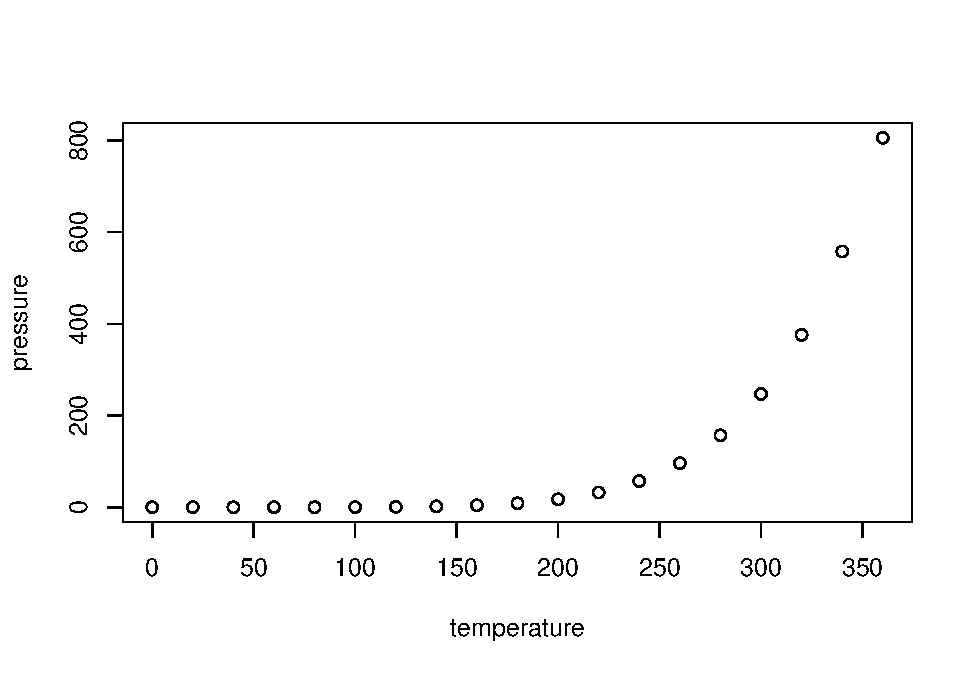
\includegraphics{firstName-lastName_StatThesis_files/figure-latex/pressure-1} \end{center}

Note that the \texttt{echo=FALSE} parameter was added to the code chunk to prevent printing of the \textbf{R} code that generated the plot. There are plenty of other ways to add chunk options. More information is available at \url{http://yihui.name/knitr/options/}.

Another useful chunk option is the setting of \texttt{cache=TRUE} as you see here. If document rendering becomes time consuming due to long computations or plots that are expensive to generate you can use knitr caching to improve performance. Later in this file, you'll see a way to reference plots created in \textbf{R} or external figures.

\hypertarget{loading-and-exploring-data}{%
\section{Loading and exploring data}\label{loading-and-exploring-data}}

Included in this template is a file called \texttt{flights.csv}. This file includes a subset of the larger dataset of information about all flights that departed from Seattle and Portland in 2014. More information about this dataset and its \textbf{R} package is available at \url{http://github.com/ismayc/pnwflights14}. This subset includes only Portland flights and only rows that were complete with no missing values. Merges were also done with the \texttt{airports} and \texttt{airlines} data sets in the \texttt{pnwflights14} package to get more descriptive airport and airline names.

We can load in this data set using the following command:
\begin{Shaded}
\begin{Highlighting}[]
\NormalTok{flights <-}\StringTok{ }\KeywordTok{read.file}\NormalTok{(}\StringTok{"data/flights.csv"}\NormalTok{)}
\end{Highlighting}
\end{Shaded}
\begin{verbatim}
   Reading data with read.csv()
\end{verbatim}
The data is now stored in the data frame called \texttt{flights} in \textbf{R}. To get a better feel for the variables included in this dataset we can use a variety of functions. Here we can see the dimensions (rows by columns) and also the names of the columns.
\begin{Shaded}
\begin{Highlighting}[]
\KeywordTok{dim}\NormalTok{(flights)}
\end{Highlighting}
\end{Shaded}
\begin{verbatim}
   [1] 52808    16
\end{verbatim}
\begin{Shaded}
\begin{Highlighting}[]
\KeywordTok{names}\NormalTok{(flights)}
\end{Highlighting}
\end{Shaded}
\begin{verbatim}
    [1] "month"        "day"          "dep_time"     "dep_delay"   
    [5] "arr_time"     "arr_delay"    "carrier"      "tailnum"     
    [9] "flight"       "dest"         "air_time"     "distance"    
   [13] "hour"         "minute"       "carrier_name" "dest_name"
\end{verbatim}
\begin{Shaded}
\begin{Highlighting}[]
\CommentTok{# read long paragraph file}
\NormalTok{longtext <-}\StringTok{ }\KeywordTok{readLines}\NormalTok{(}\StringTok{"data/paragraphs.txt"}\NormalTok{)}
\end{Highlighting}
\end{Shaded}
\begin{verbatim}
   Warning in readLines("data/paragraphs.txt"): incomplete final
   line found on 'data/paragraphs.txt'
\end{verbatim}
\begin{Shaded}
\begin{Highlighting}[]
\CommentTok{# display text as vector}
\NormalTok{longtext}
\end{Highlighting}
\end{Shaded}
\begin{verbatim}
   [1] "Lorem ipsum dolor sit amet, consectetur adipiscing elit,
   sed do eiusmod tempor incididunt ut labore et dolore magna
   aliqua. Ut enim ad minim veniam, quis nostrud exercitation
   ullamco laboris nisi ut aliquip ex ea commodo consequat. "
   [2] ""
   [3] "Duis aute irure dolor in reprehenderit in voluptate
   velit esse cillum dolore eu fugiat nulla pariatur. Excepteur
   sint occaecat cupidatat non proident, sunt in culpa qui
   officia deserunt mollit anim id est laborum."
\end{verbatim}
\begin{Shaded}
\begin{Highlighting}[]
\CommentTok{# display text as paragraphs}
\KeywordTok{cat}\NormalTok{(longtext)}
\end{Highlighting}
\end{Shaded}
\begin{verbatim}
   Lorem ipsum dolor sit amet, consectetur adipiscing elit, sed
   do eiusmod tempor incididunt ut labore et dolore magna
   aliqua. Ut enim ad minim veniam, quis nostrud exercitation
   ullamco laboris nisi ut aliquip ex ea commodo consequat.
   Duis aute irure dolor in reprehenderit in voluptate velit
   esse cillum dolore eu fugiat nulla pariatur. Excepteur sint
   occaecat cupidatat non proident, sunt in culpa qui officia
   deserunt mollit anim id est laborum.
\end{verbatim}
\begin{Shaded}
\begin{Highlighting}[]
\CommentTok{# display text without linewidth option specified}
\NormalTok{longtext}
\end{Highlighting}
\end{Shaded}
\begin{verbatim}
   [1] "Lorem ipsum dolor sit amet, consectetur adipiscing elit, sed do eiusmod tempor incididunt ut labore et dolore magna aliqua. Ut enim ad minim veniam, quis nostrud exercitation ullamco laboris nisi ut aliquip ex ea commodo consequat. "
   [2] ""                                                                                                                                                                                                                                        
   [3] "Duis aute irure dolor in reprehenderit in voluptate velit esse cillum dolore eu fugiat nulla pariatur. Excepteur sint occaecat cupidatat non proident, sunt in culpa qui officia deserunt mollit anim id est laborum."
\end{verbatim}
Another good idea is to take a look at the dataset in table form. With this dataset having more than 50,000 rows, we won't explicitly show the results of the command here. I recommend you enter the command into the Console \textbf{\emph{after}} you have run the \textbf{R} chunks above to load the data into \textbf{R}.
\begin{Shaded}
\begin{Highlighting}[]
\KeywordTok{View}\NormalTok{(flights)}
\end{Highlighting}
\end{Shaded}
While not required, it is highly recommended you use the \texttt{dplyr} package to manipulate and summarize your data set as needed. It uses a syntax that is easy to understand using chaining operations. Below I've created a few examples of using \texttt{dplyr} to get information about the Portland flights in 2014. You will also see the use of the \texttt{ggplot2} package, which produces beautiful, high-quality academic visuals.

The example we show here does the following:
\begin{itemize}
\item
  Selects only the \texttt{carrier\_name} and \texttt{arr\_delay} from the \texttt{flights} dataset and then assigns this subset to a new variable called \texttt{flights2}.
\item
  Using \texttt{flights2}, we determine the largest arrival delay for each of the carriers.
\end{itemize}
\begin{Shaded}
\begin{Highlighting}[]
\NormalTok{flights2 <-}\StringTok{ }\NormalTok{flights }\OperatorTok\StringTok{ }
\StringTok{  }\KeywordTok{select}\NormalTok{(carrier_name, arr_delay)}
\NormalTok{max_delays <-}\StringTok{ }\NormalTok{flights2 }\OperatorTok\StringTok{ }
\StringTok{  }\KeywordTok{group_by}\NormalTok{(carrier_name) }\OperatorTok
\StringTok{  }\KeywordTok{summarize}\NormalTok{(}\DataTypeTok{max_arr_delay =} \KeywordTok{max}\NormalTok{(arr_delay, }\DataTypeTok{na.rm =} \OtherTok{TRUE}\NormalTok{))}
\end{Highlighting}
\end{Shaded}
A useful function in the \texttt{knitr} package for making nice tables in \emph{R Markdown} is called \texttt{kable}. It is much easier to use than manually entering values into a table by copying and pasting values into Excel or LaTeX. This again goes to show how nice reproducible documents can be! (Note the use of \texttt{results="asis"}, which will produce the table instead of the code to create the table.) The \texttt{caption.short} argument is used to include a shorter title to appear in the List of Tables.
\begin{Shaded}
\begin{Highlighting}[]
\KeywordTok{kable}\NormalTok{(max_delays, }
      \DataTypeTok{col.names =} \KeywordTok{c}\NormalTok{(}\StringTok{"Airline"}\NormalTok{, }\StringTok{"Max Arrival Delay"}\NormalTok{),}
      \DataTypeTok{caption =} \StringTok{"Maximum Delays by Airline"}\NormalTok{,}
      \DataTypeTok{caption.short =} \StringTok{"Max Delays by Airline"}\NormalTok{,}
      \DataTypeTok{longtable =} \OtherTok{TRUE}\NormalTok{,}
      \DataTypeTok{booktabs =} \OtherTok{TRUE}\NormalTok{)}
\end{Highlighting}
\end{Shaded}
\begin{longtable}[t]{lr}
\caption[Max Delays by Airline]{\label{tab:maxdelays}Maximum Delays by Airline}\\
\toprule
Airline & Max Arrival Delay\\
\midrule
Alaska Airlines Inc. & 338\\
American Airlines Inc. & 1539\\
Delta Air Lines Inc. & 651\\
Frontier Airlines Inc. & 575\\
Hawaiian Airlines Inc. & 407\\
\addlinespace
JetBlue Airways & 273\\
SkyWest Airlines Inc. & 421\\
Southwest Airlines Co. & 694\\
United Air Lines Inc. & 472\\
US Airways Inc. & 347\\
\addlinespace
Virgin America & 366\\
\bottomrule
\end{longtable}
The last two options make the table a little easier-to-read.

We can further look into the properties of the largest value here for American Airlines Inc.~To do so, we can isolate the row corresponding to the arrival delay of 1539 minutes for American in our original \texttt{flights} dataset.
\begin{Shaded}
\begin{Highlighting}[]
\NormalTok{flights }\OperatorTok\StringTok{ }\KeywordTok{filter}\NormalTok{(arr_delay }\OperatorTok{==}\StringTok{ }\DecValTok{1539}\NormalTok{, }
\NormalTok{                  carrier_name }\OperatorTok{==}\StringTok{ "American Airlines Inc."}\NormalTok{) }\OperatorTok
\StringTok{  }\KeywordTok{select}\NormalTok{(}\OperatorTok{-}\KeywordTok{c}\NormalTok{(month, day, carrier, dest_name, hour, }
\NormalTok{            minute, carrier_name, arr_delay))}
\end{Highlighting}
\end{Shaded}
\begin{verbatim}
     dep_time dep_delay arr_time tailnum flight dest air_time
   1     1403      1553     1934  N595AA   1568  DFW      182
     distance
   1     1616
\end{verbatim}
We see that the flight occurred on March 3rd and departed a little after 2 PM on its way to Dallas/Fort Worth. Lastly, we show how we can visualize the arrival delay of all departing flights from Portland on March 3rd against time of departure.
\begin{Shaded}
\begin{Highlighting}[]
\NormalTok{flights }\OperatorTok\StringTok{ }\KeywordTok{filter}\NormalTok{(month }\OperatorTok{==}\StringTok{ }\DecValTok{3}\NormalTok{, day }\OperatorTok{==}\StringTok{ }\DecValTok{3}\NormalTok{) }\OperatorTok
\StringTok{  }\KeywordTok{ggplot}\NormalTok{(}\KeywordTok{aes}\NormalTok{(}\DataTypeTok{x =}\NormalTok{ dep_time, }\DataTypeTok{y =}\NormalTok{ arr_delay)) }\OperatorTok{+}\StringTok{ }\KeywordTok{geom_point}\NormalTok{()}
\end{Highlighting}
\end{Shaded}
\begin{center}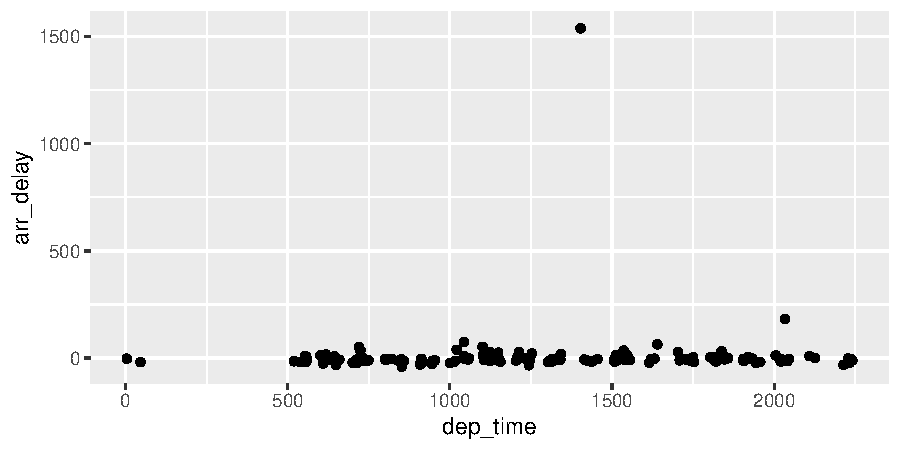
\includegraphics{firstName-lastName_StatThesis_files/figure-latex/march3plot-1} \end{center}
\begin{proof}[This is a proof]
\iffalse{} {Proof (This is a proof). } \fi{}There is a proof environment in which you can create equations

\[
\hat{\beta}_0 + \hat{\beta}_1x
\]
\end{proof}
\hypertarget{additional-resources}{%
\section{Additional resources}\label{additional-resources}}
\begin{itemize}
\item
  \emph{Markdown} Cheatsheet - \url{https://github.com/adam-p/markdown-here/wiki/Markdown-Cheatsheet}
\item
  \emph{R Markdown} Reference Guide - \url{https://www.rstudio.com/wp-content/uploads/2015/03/rmarkdown-reference.pdf}
\item
  Introduction to \texttt{dplyr} - \url{https://cran.rstudio.com/web/packages/dplyr/vignettes/introduction.html}
\item
  \texttt{ggplot2} Documentation - \url{http://docs.ggplot2.org/current/}
\end{itemize}
\hypertarget{math-sci}{%
\chapter{Mathematics and Science}\label{math-sci}}

\hypertarget{math}{%
\section{Math}\label{math}}

\TeX~is the best way to typeset mathematics. Donald Knuth designed \TeX~when he got frustrated at how long it was taking the typesetters to finish his book, which contained a lot of mathematics. One nice feature of \emph{R Markdown} is its ability to read LaTeX code directly.

If you are doing a thesis that will involve lots of math, you will want to read the following section.

\[
\sum_{j=1}^n (\delta\theta_j)^2 \leq 
\frac{\beta_i^2}{\delta_i^2 + \rho_i^2}
\left[ 2\rho_i^2 + \frac{\delta_i^2\beta_i^2}{\delta_i^2 + \rho_i^2} \right] \equiv \omega_i^2
\]

From Informational Dynamics, we have the following (Dave Braden):

After \emph{n} such encounters the posterior density for \(\theta\) is

\[
\pi(\theta|X_1< y_1,\dots,X_n<y_n) \varpropto \pi(\theta) \prod_{i=1}^n\int_{-\infty}^{y_i}
   \exp\left(-\frac{(x-\theta)^2}{2\sigma^2}\right)\ dx
\]

Another equation:

\[
\det\left|\,\begin{matrix}%
c_0&c_1\hfill&c_2\hfill&\ldots&c_n\hfill\cr
c_1&c_2\hfill&c_3\hfill&\ldots&c_{n+1}\hfill\cr
c_2&c_3\hfill&c_4\hfill&\ldots&c_{n+2}\hfill\cr
\,\vdots\hfill&\,\vdots\hfill&
  \,\vdots\hfill&&\,\vdots\hfill\cr
c_n&c_{n+1}\hfill&c_{n+2}\hfill&\ldots&c_{2n}\hfill\cr
\end{matrix}\right|>0
\]

\hypertarget{statistics-symbols-and-expressions}{%
\section{Statistics Symbols and Expressions}\label{statistics-symbols-and-expressions}}

\noindent Exponent or Superscript: \(x^2\)

\noindent Subscript: \(x_1, x_2, \dots, x_n\)

\noindent Both combined: \(x_1^{k+1}\).

\noindent Our favorite Greeks: \(\sigma\), \(\epsilon\), \(\mu\)

\noindent Defining a normally distributed random variable: \(X\sim N(\mu, \sigma)\)

How do we compute sample variance again?

\[s^2 = \frac{\sum_{i=1}^n (x_i-\bar x)^2}{n-1}\]

Sometimes you'll need to consider asymptotics, that is, what happens as \(n\rightarrow \infty\).

\hypertarget{additional-information}{%
\section{Additional information}\label{additional-information}}

Many of the symbols you will need can be found on Reed College's math page \url{http://web.reed.edu/cis/help/latex/math.html} and the Comprehensive LaTeX Symbol Guide (\url{http://mirror.utexas.edu/ctan/info/symbols/comprehensive/symbols-letter.pdf}).

\hypertarget{ref-labels}{%
\chapter{Tables, Graphics, References, and Labels}\label{ref-labels}}

\hypertarget{tables}{%
\section{Tables}\label{tables}}

In addition to the tables that can be automatically generated from a data frame in \textbf{R} that you saw in \protect\hyperlink{rmd-basics}{R Markdown Basics} using the \texttt{kable} function, you can also create tables using \emph{pandoc}. (More information is available at \url{http://pandoc.org/README.html\#tables}.) This might be useful if you don't have values specifically stored in \textbf{R}, but you'd like to display them in table form. Below is an example. Pay careful attention to the alignment in the table and hyphens to create the rows and columns.
\begin{longtable}[]{@{}ccc@{}}
\caption{\label{tab:inher} Correlation of Inheritance Factors for Parents and Child}\tabularnewline
\toprule
\begin{minipage}[b]{0.29\columnwidth}\centering
Factors\strut
\end{minipage} & \begin{minipage}[b]{0.46\columnwidth}\centering
Correlation between Parents \& Child\strut
\end{minipage} & \begin{minipage}[b]{0.16\columnwidth}\centering
Inherited\strut
\end{minipage}\tabularnewline
\midrule
\endfirsthead
\toprule
\begin{minipage}[b]{0.29\columnwidth}\centering
Factors\strut
\end{minipage} & \begin{minipage}[b]{0.46\columnwidth}\centering
Correlation between Parents \& Child\strut
\end{minipage} & \begin{minipage}[b]{0.16\columnwidth}\centering
Inherited\strut
\end{minipage}\tabularnewline
\midrule
\endhead
\begin{minipage}[t]{0.29\columnwidth}\centering
Education\strut
\end{minipage} & \begin{minipage}[t]{0.46\columnwidth}\centering
-0.49\strut
\end{minipage} & \begin{minipage}[t]{0.16\columnwidth}\centering
Yes\strut
\end{minipage}\tabularnewline
\begin{minipage}[t]{0.29\columnwidth}\centering
Socio-Economic Status\strut
\end{minipage} & \begin{minipage}[t]{0.46\columnwidth}\centering
0.28\strut
\end{minipage} & \begin{minipage}[t]{0.16\columnwidth}\centering
Slight\strut
\end{minipage}\tabularnewline
\begin{minipage}[t]{0.29\columnwidth}\centering
Income\strut
\end{minipage} & \begin{minipage}[t]{0.46\columnwidth}\centering
0.08\strut
\end{minipage} & \begin{minipage}[t]{0.16\columnwidth}\centering
No\strut
\end{minipage}\tabularnewline
\begin{minipage}[t]{0.29\columnwidth}\centering
Family Size\strut
\end{minipage} & \begin{minipage}[t]{0.46\columnwidth}\centering
0.18\strut
\end{minipage} & \begin{minipage}[t]{0.16\columnwidth}\centering
Slight\strut
\end{minipage}\tabularnewline
\begin{minipage}[t]{0.29\columnwidth}\centering
Occupational Prestige\strut
\end{minipage} & \begin{minipage}[t]{0.46\columnwidth}\centering
0.21\strut
\end{minipage} & \begin{minipage}[t]{0.16\columnwidth}\centering
Slight\strut
\end{minipage}\tabularnewline
\bottomrule
\end{longtable}
We can also create a link to the table by doing the following: Table \ref{tab:inher}. If you go back to \protect\hyperlink{loading-and-exploring-data}{Loading and exploring data} and look at the \texttt{kable} table, we can create a reference to this max delays table too: Table \ref{tab:maxdelays}. The addition of the \texttt{(\textbackslash{}\#tab:inher)} option to the end of the table caption allows us to then make a reference to Table \texttt{\textbackslash{}@ref(tab:label)}. Note that this reference could appear anywhere throughout the document after the table has appeared.

\clearpage

\hypertarget{figures}{%
\section{Figures}\label{figures}}

If your thesis has a lot of figures, \emph{R Markdown} might behave better for you than that other word processor. One perk is that it will automatically number the figures accordingly in each chapter. You'll also be able to create a label for each figure, add a caption, and then reference the figure in a way similar to what we saw with tables earlier. If you label your figures, you can move the figures around and \emph{R Markdown} will automatically adjust the numbering for you. No need for you to remember! So that you don't have to get too far into LaTeX to do this, a couple \textbf{R} functions have been created for you to assist. You'll see their use below.

In the \textbf{R} chunk below, we will load in a picture stored as \texttt{amherst.png} in our main directory. We then give it the caption of ``Amherst logo'', the label of ``amherstlogo'', and specify that this is a figure. Make note of the different \textbf{R} chunk options that are given in the R Markdown file (not shown in the knitted document).
\begin{Shaded}
\begin{Highlighting}[]
\KeywordTok{include_graphics}\NormalTok{(}\DataTypeTok{path =} \StringTok{"figures/amherst.png"}\NormalTok{)}
\end{Highlighting}
\end{Shaded}
\begin{figure}

{\centering 
\includegraphics[width=0.5\linewidth]{figures/amherst} 

}

\caption{Amherst logo}\label{fig:amherstlogo}
\end{figure}
Here is a reference to the Amherst logo: Figure \ref{fig:amherstlogo}. Note the use of the \texttt{fig:} code here. By naming the \textbf{R} chunk that contains the figure, we can then reference that figure later as done in the first sentence here. We can also specify the caption for the figure via the R chunk option \texttt{fig.cap}.

\clearpage

Below we will investigate how to save the output of an \textbf{R} plot and label it in a way similar to that done above. Recall the \texttt{flights} dataset from Chapter \ref{rmd-basics}. (Note that we've shown a different way to reference a section or chapter here.) We will next explore a bar graph with the mean flight departure delays by airline from Portland for 2014. Note also the use of the \texttt{scale} parameter which is discussed on the next page.
\begin{Shaded}
\begin{Highlighting}[]
\CommentTok{#if(!exists("flights")) flights <- read.csv("data/flights.csv")}
\NormalTok{flights }\OperatorTok\StringTok{ }\KeywordTok{group_by}\NormalTok{(carrier) }\OperatorTok
\StringTok{  }\KeywordTok{summarize}\NormalTok{(}\DataTypeTok{mean_dep_delay =} \KeywordTok{mean}\NormalTok{(dep_delay)) }\OperatorTok
\StringTok{  }\KeywordTok{ggplot}\NormalTok{(}\KeywordTok{aes}\NormalTok{(}\DataTypeTok{x =}\NormalTok{ carrier, }\DataTypeTok{y =}\NormalTok{ mean_dep_delay)) }\OperatorTok{+}
\StringTok{  }\KeywordTok{geom_bar}\NormalTok{(}\DataTypeTok{position =} \StringTok{"identity"}\NormalTok{, }\DataTypeTok{stat =} \StringTok{"identity"}\NormalTok{, }\DataTypeTok{fill =} \StringTok{"red"}\NormalTok{)}
\end{Highlighting}
\end{Shaded}
\begin{figure}

{\centering 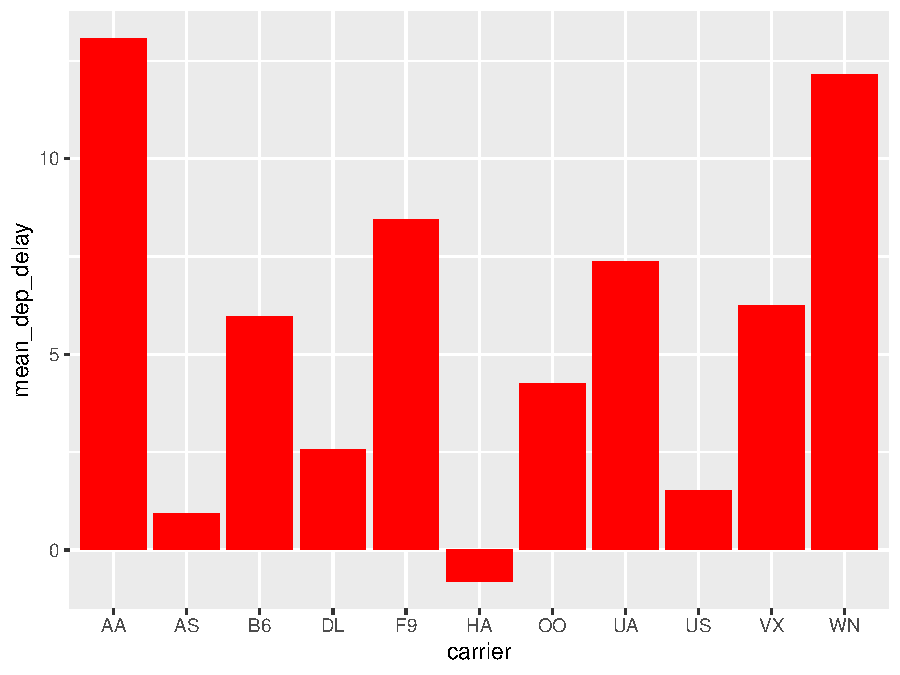
\includegraphics{firstName-lastName_StatThesis_files/figure-latex/delaysboxplot-1} 

}

\caption{Mean Delays by Airline}\label{fig:delaysboxplot}
\end{figure}
Here is a reference to this image: Figure \ref{fig:delaysboxplot}.

A table linking these carrier codes to airline names is available at \url{https://github.com/ismayc/pnwflights14/blob/master/data/airlines.csv}.

\clearpage

Next, we will explore the use of the \texttt{out.extra} chunk option, which can be used to shrink or expand an image loaded from a file by specifying \texttt{"scale=\ "}. Here we use the mathematical graph stored in the ``subdivision.pdf'' file.
\begin{figure}

{\centering 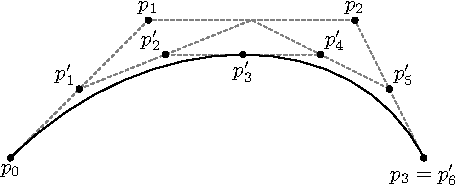
\includegraphics[scale=0.75]{figures/subdivision} 

}

\caption{Subdiv. graph}\label{fig:subd}
\end{figure}
Here is a reference to this image: Figure \ref{fig:subd}. Note that \texttt{echo=FALSE} is specified so that the \textbf{R} code is hidden in the document.

\textbf{More Figure Stuff}

Lastly, we will explore how to rotate and enlarge figures using the \texttt{out.extra} chunk option. (Currently this only works in the PDF version of the book.)
\begin{figure}

{\centering 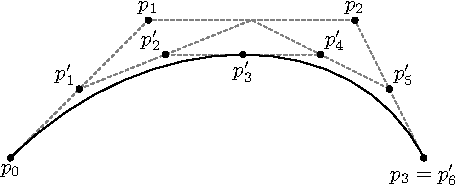
\includegraphics[angle=180, scale=1.1]{figures/subdivision} 

}

\caption{A Larger Figure, Flipped Upside Down}\label{fig:subd2}
\end{figure}
As another example, here is a reference: Figure \ref{fig:subd2}.

\hypertarget{footnotes-and-endnotes}{%
\section{Footnotes and Endnotes}\label{footnotes-and-endnotes}}

You might want to footnote something.\footnote{footnote text} The footnote will be in a smaller font and placed appropriately. Endnotes work in much the same way. More information can be found about both on the Reed Thesis site \url{https://www.reed.edu/cis/help/latex/thesis.html} or feel free to reach out to Prof.~Bailey at \href{mailto:bebailey@amherst.edu}{\nolinkurl{bebailey@amherst.edu}}.

\hypertarget{bibliographies}{%
\section{Bibliographies}\label{bibliographies}}

Of course you will need to cite things, and you will probably accumulate an armful of sources. There are a variety of tools available for creating a bibliography database (stored with the .bib extension). In addition to BibTeX suggested below, you may want to consider using the free and easy-to-use tool called Zotero. The Amherst librarians have created Zotero documentation at \url{https://www.amherst.edu/library/find/citation/zotero}. In addition, a tutorial is available from Middlebury College at \url{http://sites.middlebury.edu/zoteromiddlebury/}.

\emph{R Markdown} uses \emph{pandoc} (\url{http://pandoc.org/}) to build its bibliographies. One nice caveat of this is that you won't have to do a second compile to load in references as standard LaTeX requires. To cite references in your thesis (after creating your bibliography database), place the reference name inside square brackets and precede it by the ``at'' symbol. For example, here's a reference to a book about worrying: (Molina \& Borkovec, 1994). This \texttt{Molina1994} entry appears in a file called \texttt{thesis.bib} in the \texttt{bib} folder. This bibliography database file was created by a program called BibTeX. You can call this file something else if you like (look at the YAML header in the main .Rmd file) and, by default, is to placed in the \texttt{bib} folder.

For more information about BibTeX and bibliographies, see the Reed College CUS site (\url{http://web.reed.edu/cis/help/latex/index.html})\footnote{Reed~College (2007)}. There are three pages on this topic: \emph{bibtex} (which talks about using BibTeX, at \url{http://web.reed.edu/cis/help/latex/bibtex.html}), \emph{bibtexstyles} (about how to find and use the bibliography style that best suits your needs, at \url{http://web.reed.edu/cis/help/latex/bibtexstyles.html}) and \emph{bibman} (which covers how to make and maintain a bibliography by hand, without BibTeX, at \url{http://web.reed.edu/cis/help/latex/bibman.html}). The last page will not be useful unless you have only a few sources.

If you look at the YAML header at the top of the main .Rmd file you can see that we can specify the style of the bibliography by referencing the appropriate csl file. You can download a variety of different style files at \url{https://www.zotero.org/styles}. Make sure to download the file into the csl folder.

\textbf{Tips for Bibliographies}
\begin{itemize}
\tightlist
\item
  Like with thesis formatting, the sooner you start compiling your bibliography for something as large as thesis, the better. Typing in source after source is mind-numbing enough; do you really want to do it for hours on end in late April? Think of it as procrastination.
\item
  The cite key (a citation's label) needs to be unique from the other entries.
\item
  When you have more than one author or editor, you need to separate each author's name by the word ``and'' e.g.~\texttt{Author\ =\ \{Noble,\ Sam\ and\ Youngberg,\ Jessica\},}.
\item
  Bibliographies made using BibTeX (whether manually or using a manager) accept LaTeX markup, so you can italicize and add symbols as necessary.
\item
  To force capitalization in an article title or where all lowercase is generally used, bracket the capital letter in curly braces.
\item
  You can add a Reed Thesis citation\footnote{Noble (2002)} option. The best way to do this is to use the phdthesis type of citation, and use the optional ``type'' field to enter ``Reed thesis'' or ``Undergraduate thesis.''
\end{itemize}
\hypertarget{anything-else}{%
\section{Anything else?}\label{anything-else}}

If you'd like to see examples of other things in this template, please contact Professor Bailey (email \href{mailto:bebailey@amherst.edu}{\nolinkurl{bebailey@amherst.edu}}) with your suggestions.

\hypertarget{conclusion-1}{%
\chapter*{Conclusion}\label{conclusion-1}}
\addcontentsline{toc}{chapter}{Conclusion}

If we don't want the conclusion to have a chapter number next to it, we can add the \texttt{\{-\}} attribute.

\textbf{More info}

And here's some other random info: the first paragraph after a chapter title or section head \emph{shouldn't be} indented, because indents are to tell the reader that you're starting a new paragraph. Since that's obvious after a chapter or section title, proper typesetting doesn't add an indent there.

\appendix

\hypertarget{the-first-appendix}{%
\chapter{The First Appendix}\label{the-first-appendix}}

This first appendix includes all of the R chunks of code that were hidden throughout the document (using the \texttt{include\ =\ FALSE} chunk tag) to help with readibility and/or setup.

\hypertarget{in-the-main-file-refref-labels}{%
\section{In the main file \ref{ref-labels}:}\label{in-the-main-file-refref-labels}}

\hypertarget{in-chapter-refref-labels}{%
\section{In Chapter \ref{ref-labels}:}\label{in-chapter-refref-labels}}

\hypertarget{the-second-appendix}{%
\chapter{The Second Appendix}\label{the-second-appendix}}

R code

\hypertarget{corrections}{%
\chapter*{Corrections}\label{corrections}}
\addcontentsline{toc}{chapter}{Corrections}

A list of corrections after submission to department.

Corrections may be made to the body of the thesis, but every such correction will be acknowledged in a list under the heading ``Corrections,'' along with the statement ``When originally submitted, this honors thesis contained some errors which have been corrected in the current version. Here is a list of the errors that were corrected.'' This list will be given on a sheet or sheets to be appended to the thesis. Corrections to spelling, grammar, or typography may be acknowledged by a general statement such as ``30 spellings were corrected in various places in the thesis, and the notation for definite integral was changed in approximately 10 places.'' However, any correction that affects the meaning of a sentence or paragraph should be described in careful detail. The files samplethesis.tex and samplethesis.pdf show what the ``Corrections'' section should look like. Questions about what should appear in the ``Corrections'' should be directed to the Chair.

\backmatter

\hypertarget{references}{%
\chapter*{References}\label{references}}
\addcontentsline{toc}{chapter}{References}

\noindent

\setlength{\parindent}{-0.20in}
\setlength{\leftskip}{0.20in}
\setlength{\parskip}{8pt}

\hypertarget{refs}{}
\leavevmode\hypertarget{ref-angel2000}{}%
Angel, E. (2000). \emph{Interactive computer graphics : A top-down approach with opengl}. Boston, MA: Addison Wesley Longman.

\leavevmode\hypertarget{ref-angel2001}{}%
Angel, E. (2001a). \emph{Batch-file computer graphics : A bottom-up approach with quicktime}. Boston, MA: Wesley Addison Longman.

\leavevmode\hypertarget{ref-angel2002a}{}%
Angel, E. (2001b). \emph{Test second book by angel}. Boston, MA: Wesley Addison Longman.

\leavevmode\hypertarget{ref-Molina1994}{}%
Molina, S. T., \& Borkovec, T. D. (1994). The Penn State worry questionnaire: Psychometric properties and associated characteristics. In G. C. L. Davey \& F. Tallis (Eds.), \emph{Worrying: Perspectives on theory, assessment and treatment} (pp. 265--283). New York: Wiley.

\leavevmode\hypertarget{ref-noble2002}{}%
Noble, S. G. (2002). \emph{Turning images into simple line-art} (Undergraduate thesis). Reed College.

\leavevmode\hypertarget{ref-reedweb2007}{}%
Reed~College. (2007). LaTeX your document. Retrieved from \url{http://web.reed.edu/cis/help/LaTeX/index.html}

% Index?

\end{document}
